
\section{The Tableau}\label{sec:tableau}


We decide satisfiability of an input formula $\varphi$ by a depth-first, on-the-fly construction that builds
a graph of symbolic nodes and searches it for a {successful marking}. A node carries the
formulas to be realised at a configuration; zones represent clock valuations symbolically; and a single
{cover} rule discharges every time-bounded modality. We fix nodes and realisability (\S\ref{ss:nodes}), give the rules (\S\ref{ss:rules}), define
acceptance and its test (\S\ref{ss:loop}), and close with two examples (\S\ref{ss:ex}).

\subsection{Nodes and Realisability}\label{ss:nodes}


A {node} is a tuple $N=\tup{\Gamma}{\Ctx}{Z}{\obligations}{\Deadline}$, where $\Gamma$ is the set of
goal formulas to be satisfied (write $\Gamma_{\mathsf{prop}}=\Gamma\cap\big(\mathcal P\cup\{\neg p\mid p\in\mathcal P\}\big)$ for the propositional part); $\Ctx$ the {context} of universal formulas that must
hold at every successor; $Z$ the set of clock valuations for this node, represented as a canonical zone; $\obligations$ the {clock map}, which allocates to every active timed modality $\mu$ a dedicated formula-clock $x_\mu$ so its window (i.e. its interval \kI) can be measured from the configuration that demanded it; and $\Deadline$ is a set of deadlines
$(x_\mu,\sup\kI)$, each with a strictness flag, and $\Inv(N)=\bigwedge_{(x_\mu,b)\in \Deadline}x_\mu\le b$
its induced invariant.

%A deadline is added when \ruleref{Cov} launches the pursuit of a
%universal until and removed when the $(\text{stop})$ branch of \ruleref{Uunf} discharges it;
%no other rule writes $\Deadline$.
%
%; and $\eventualities$ the postponed eventualities used for loopacceptance. 


%Write $\Gamma_{\mathsf{prop}}=\Gamma\cap\big(\mathcal P\cup\{\neg p\mid p\in\mathcal P\}\big)$ for the {propositional part} of $\Gamma$, the atomic literals it asserts. A node is {closed} if $\Gamma_{\mathsf{prop}}$ is propositionally inconsistent, i.e., it contains a complementary pair $p,\neg p$ (equivalently $\bot\in\Gamma$), or its zone is empty, $Z=\emptyset$; it is {saturated} when no expansion rule applies.



%\noindent
%We write
%$\Gamma_{\mathsf{prop}}=\Gamma\cap\big(\mathcal P\cup\{\neg p\mid p\in\mathcal P\}\big)$ for the
%\emph{propositional part} of $\Gamma$, the atomic literals it asserts. 

We call a sequence of nodes $N_0,N_1,\dots$ a \emph{path} if each $N_{i+1}$ is a child of $N_i$. 
%Write
%\[
%  \Inv(N)\hspace{-0.1cm}=\hspace{-0.1cm}\bigwedge\big\{x_\mu\le\sup\kI \big| \mu=\mathrm{A}(\varphi\,\mathbf{U}_\kI\,\psi)
%  \text{ under pursuit at } N \big\} \quad (<\text{ if } \sup\kI\notin\kI)
%\]
%for the node's {invariant}. Both $x_\mu$ and the bound are read off the node: the clock
%from $\obligations$, the interval from $\mu$ itself.
%
%$\clocks(\obligations)$
A node is \emph{closed} if $\Gamma_{\mathsf{prop}}$ is propositionally inconsistent, i.e. it contains a
complementary pair $p,\neg p$ (equivalently $\bot\in\Gamma$), or its zone is empty, $Z=\emptyset$. It is
\emph{saturated} when no saturation or cover rule applies; only saturated nodes generate successors.
It is \emph{realisable} if there is a non-blocking TTS $\mathcal T$ induced by a TA, a location $s$ with
$L(s)\supseteq\Gamma_{\mathsf{prop}}$ and $\Inv(s)=\Inv(N)$, and an interpretation of the
formula-clocks in \obligations, such that for every $\nu \in Z$ the configuration $(s,\nu)$  $\mathcal T,(s,\nu)\models\textstyle\bigwedge\Gamma\ \wedge\ \bigwedge\Ctx$. Realisability is \emph{monotone under narrowing}: if $\tup{\Gamma}{\Ctx}{Z}{\obligations}{\Deadline}$ is realisable and
$\emptyset\neq Z'\subseteq Z$, then $\tup{\Gamma}{\Ctx}{Z'}{\obligations}{\Deadline}$ is realisable.


%Two consequences of Definition~\ref{def:realisable} shape the calculus. First, the quantification over $Z$ is \emph{universal}: this is precisely what lets a single node discharge a demand re-imposed by a persistent context at a continuum of onsets. Second, realisability is \emph{monotone under narrowing}.

%\begin{lemma}[Narrowing]\label{lem:narrowing}
%If $\tup{\Gamma}{\Ctx}{Z}{\obligations}$ is realisable and
%$\emptyset\neq Z'\subseteq Z$, then $\tup{\Gamma}{\Ctx}{Z'}{\obligations}$ is realisable.
%\end{lemma}
%\begin{proof}
%Immediate: the condition of Definition~\ref{def:realisable} is universally quantified over the zone, and
%$Z'$ is a non-empty subset of $Z$.
%\end{proof}
%
%Lemma~\ref{lem:narrowing} is what licenses the refinement rule \ruleref{Covstar} to be a disjunctive
%choice rather than a case analysis: a node is free to commit to a tighter entry constraint. For this to
%be sound at the level of the extracted automaton, the narrowing must happen \emph{before} the node's
%outgoing steps are fixed; this is guaranteed by the discipline of \S\ref{ss:rules}, where a node is
%saturated and covered to exhaustion before any successor is generated, so the guards of its delays and
%edges are read off the narrowed zone.

%\noindent
The construction branches two ways. An \emph{OR} (disjunctive, $\ORn$) node is realisable if
\emph{some} child is; an \emph{AND} (conjunctive, $\ANDn$) node requires \emph{all} its children. Some
rules are deterministic ($\DETn$): a single child, replacing the node. 


%Table~\ref{tab:rulekinds} fixes the kind of every rule; the marginal marker on each rule below repeats it.

%\begin{table}[t]
%\centering
%\caption{Every rule and its branching kind. $\DETn$ = single child, $\ORn$ = OR-node,
%$\ANDn$ = AND-node.}\label{tab:rulekinds}
%\begin{tabular}{llll}
%\hline
%Group & Rule & Kind & Children \\
%\hline
%Saturation & $(\wedge)$, \ruleref{AX} & $\DETn$ & $1$ \\
%Saturation & $(\vee)$ & $\ORn$ & $2$ \\
%Cover & \ruleref{Cov} & $\ANDn$ & $2$ (discharge, launch) \\
%Cover & \ruleref{Covstar} & $\ORn$ & one per convex component \\
%Pursuit & \ruleref{Uunf} & $\ORn$ & $2$ (stop, go) \\
%Pursuit & \ruleref{Rsplit} & $\ANDn$ & $\le 3$ (before, in, after) \\
%Pursuit & \ruleref{Runf} & $\ORn$ & $2$ per part \\
%Successors & \ruleref{Delay} & $\ANDn$ & $2$ (open segment, boundary) \\
%Successors & \ruleref{EX} & $\ANDn$ & one per $\EX\psi\in\Gamma$, or stutter \\
%\hline
%\end{tabular}
%\end{table}
%
\noindent


%A \emph{marking} $\mathcal M$ selects one child at each OR-node and \emph{all} children at each
%AND-node; it is \emph{successful} if it contains no closed node and every postponed eventuality is
%fulfilled on every infinite path, in the sense made effective by the loop condition of
%\S\ref{ss:loop}. 



%The tableau \emph{succeeds} on $\varphi$ if the root
%$\tup{\{\varphi\}}{\emptyset}{\Zuniv}{\emptyset}{\emptyset}$ admits a successful marking, where
%$\Zuniv$ is the universal zone over $\clockSet$.

%
%\subsection{Satisfaction sets}\label{ss:sat}
%
%The cover rule consults, for a timed modality $\mu$ demanded under context $\Ctx$, the set
%$\Sat_{\Ctx}(\mu)\subseteq\mathbb{R}^{\clockSet\cup\{x_\mu\}}_{\ge0}$ of valuations at which $\mu$ holds
%under that context. We compute it at the logical level, without assuming a model, by \emph{pursuing}
%$\mu$: a fresh formula-clock $x_\mu$ is reset where the demand arises and measures elapsed time against
%$\kI$, and the pursued modality --- written $\mu^\bullet$ --- is unfolded one step at a time by the
%rules \ruleref{Uunf}, \ruleref{Rsplit} and \ruleref{Runf} of \S\ref{ss:rules}.
%
%Each unfolding step produces two kinds of child. A \emph{base} child settles the demand at once and drops
%$\mu^\bullet$; the union of the base zones is written $B_\mu$. A \emph{recursive} child defers it,
%propagating $\nxQ\mu^\bullet$ to the successors, where
%\[
%  \nxQ\mu^\bullet \;=\;
%  \begin{cases}
%    \EX\mu^\bullet \text{ placed in } \Gamma, & \mathrm{Q}=\mathrm{E},\\[2pt]
%    \AX\mu^\bullet \text{ placed in } \Ctx,   & \mathrm{Q}=\mathrm{A},
%  \end{cases}
%\]
%so that an existential pursuit travels as a goal and demands \emph{one} successor, while a universal
%pursuit travels as context and is re-imposed on \emph{every} successor. Either way $x_\mu$ keeps running,
%across delays as well as edges. A valuation $\nu$ lies in $\Sat_{\Ctx}(\mu)$ exactly when it lies in
%$B_\mu$, or it matches a recursive child whose deferred successors lie in $\Sat_{\Ctx}(\mu)$ --- some
%successor when $\mathrm{Q}=\mathrm{E}$, all of them when $\mathrm{Q}=\mathrm{A}$. An until takes the
%\emph{least} solution of this equation, a valuation qualifying only if it can \emph{reach} a base child
%in finitely many steps; a release takes the \emph{greatest}, a valuation qualifying as long as it can
%continue without ever violating the release.

%\begin{remark}[Stratification]\label{rem:strat}
%The definition is not circular. $\Sat_{\Ctx}(\mu)$ is computed in a separate \emph{pursuit graph},
%generated by \ruleref{Uunf}, \ruleref{Rsplit}, \ruleref{Runf} and successor generation alone; the cover
%rule is never re-entered for $\mu$ itself. Nested modalities are resolved by induction on the
%Fischer--Ladner order: the pursuit of $\mu$ may consult $\Sat_{\Ctx}(\mu')$ only for
%$\mu'\in\FL(\mu)\setminus\{\mu\}$, already available. Within one stratum the equation is a monotone map
%on finite unions of $\cong_M$-zones, so least and greatest fixpoints exist and are reached by finite
%iteration (Knaster--Tarski over that finite lattice). In particular $\Sat_{\Ctx}(\mu)$ is a finite union
%of zones, computed in finitely many steps, and a single $x_\mu$ serves all onsets of a persistent demand,
%since the dense family of onsets is absorbed into that union.
%\end{remark}
%
\subsection{Rules}\label{ss:rules}


%Each rule rewrites a node into its children, shown on the full tuple; a component reappears unchanged unless the rule modifies it.

Rules come in four groups: \emph{saturation}
decomposes the goals in $\Gamma$, the \emph{cover} rule discharges a timed modality, the
\emph{pursuit} rules unfold a launched modality one step at a time, and \emph{successor
generation} expands a saturated node in time and across edges.

\paragraph{Saturation.}
Conjunction \ruleref{Conj} is deterministic, disjunction \ruleref{Disj} branches, and \ruleref{AX} handles a universal marker by moving its argument into the context. %There is no saturation rule for $\EX$: ``some successor satisfies
%$\psi$'' cannot be settled before successors exist, so $\EX\psi$ waits in $\Gamma$ and is discharged by
%\ruleref{EX}.
\vspace{-0.2cm}
\[
\ \frac{\tup{\Gamma\cup\{\varphi\land\psi\}}{\Ctx}{Z}{\obligations}{\Deadline}}
{\tup{\Gamma\cup\{\varphi,\psi\}}{\Ctx}{Z}{\obligations}{\Deadline}}\quad
\shortstack{\ruleanchor{Conj}\\\DETn}
\qquad
\ \frac{\tup{\Gamma\cup\{\AX\varphi\}}{\Ctx}{Z}{\obligations}{\Deadline}}
{\tup{\Gamma}{\Ctx\cup\{\varphi\}}{Z}{\obligations}{\Deadline}}\quad
\shortstack{\ruleanchor{AX}\\ \DETn}
\]\vspace{-0.35cm}
\[
\ \frac{\tup{\Gamma\cup\{\varphi\lor\psi\}}{\Ctx}{Z}{\obligations}{\Deadline}}
{\tup{\Gamma\cup\{\varphi\}}{\Ctx}{Z}{\obligations}{\Deadline}\quad\big|\quad
\tup{\Gamma\cup\{\psi\}}{\Ctx}{Z}{\obligations}{\Deadline}}
\quad
\shortstack{\ruleanchor{Disj}\\\ORn}
\]

\paragraph{The cover rule.}
When $\Gamma$ contains a timed modality $\mu=\mathrm{Q}(\varphi\,\circ_\kI\,\psi)$, with
$\mathrm{Q}\in\{\mathrm{E},\mathrm{A}\}$ and $\circ\in\{\mathbf{U},\mathbf{R}\}$, we say the node
\emph{demands} $\mu$ and it must be shown that $\mu$ holds at every
valuation of the node's zone. Since $\kI$ is measured from the demanding configuration, a persistent
context, e.g., $\mathrm{AG}(\mu)$, would issue a new demand at uncountably many configurations of the
zone; we avoid this by testing the zone symbolically. Suppose we knew the set $\Sat_{\Ctx}(\mu) \subseteq \mathbb{R}_{\ge0}^{\clockSet\cup\{x_\mu\}}$ of all clock valuations at which $\mu$ holds under \Ctx. The demand is then met exactly when the node's zone lies totally inside it, $Z\subseteq\Sat_{\Ctx}(\mu)$, in which case rule \ruleref{Cov} applies. The rule has two children: the \ruleref{discharge}, which drops $\mu$ from $\Gamma$, allowing the node to continue with the rest of $\Gamma$, and the \ruleref{launch}, which launches a \emph{pursuit} of $\mu$ (which we write $\mu^\bullet$), i.e., a new branch of the tableau that unfolds $\mu$ to find a witness, introducing a fresh formula-clock $x_\mu$ to measure the window $\kI$ from the demanding configuration. 


%(i) introduces a fresh formula-clock $x_\mu$ and resets it to zero, so that the window $\kI$ can be measured from the demanding configuration 


%which can be discharged



%The two children are conjunctive because they play different roles: the
%\emph{stop} settles $\mu$ at once, allowing the node to continue with the rest of $\Gamma$, while the \emph{go} child pursues $\mu$, which we indicate with $\mu^\bullet$. A pursuit of $\mu$ starts by introducing a fresh formula-clock $x_\mu$ and resetting it to zero, so that the window $\kI$ can be measured from the demanding configuration. 


%discharged by \ruleref{Cov}.
%The rule
%\ruleref{Cov} discharges $\mu$ when the cover is total, \ruleref{Covstar} narrows the node when it is
%partial, and the node closes when it is empty.
%
\vspace{-0.3cm}
\[
\frac{\tup{\Gamma\cup\{\mu\}}{\Ctx}{Z}{\obligations}{\Deadline}}
{\begin{array}{ll}
\tup{\Gamma}{\Ctx}{Z}{\obligations}{\Deadline} & \ruleanchor{discharge}\\[3pt]
\tup{\Gamma\cup\{\mu^\bullet\}}{\Ctx}{\rst{Z}{x_\mu}}{\obligations[\mu\mapsto x_\mu]}{\Deadline\cup \Deadline_\mu}
 & \ruleanchor{launch}
\end{array}}
\quad
\begin{array}{l}
Z\subseteq\Sat_{\Ctx}(\mu)\\
x_\mu \text{ fresh}
\end{array}
\shortstack{\ruleanchor{Cov}\\\ANDn}
\]

A deadline $\Deadline_\mu=\{(x_\mu,\sup\kI)\}$ is applied iff $\mu$ is a universal until, with $\Deadline_\mu=\emptyset$ otherwise. Only such a modality needs one, as it obliges \emph{every} run to satisfy $\psi$ within $\kI$ and time must be forced forward or a run could idle past the window with the eventuality unmet. An existential until is discharged by a single witnessing run, and a release, of either quantifier, is discharged by lapsing past the window rather than by acting within it.

%
%The cover rule applies a deadline $\Deadline_\mu=\{(x_\mu,\sup\kI)\}$ iff $\mu$ is a universal until,
%$\mu=\mathrm{A}(\varphi\,\mathbf{U}_\kI\,\psi)$, and otherwise $\Deadline_\mu=\emptyset$. Only such a
%modality needs one, as it obliges \emph{every} run to satisfy $\psi$ within $\kI$: time must be
%forced forward or a run could idle past the window with the eventuality unmet. An existential
%until is discharged by a single witnessing run, and a release, of either quantifier, is
%discharged by lapsing past the window rather than by acting within it.




%The universal deferral is additionally capped at the deadline $x_\mu\le\sup\kI$ (strict when
%$\sup\kI\notin\kI$). We record that cap in $\Inv(N)$ rather than in $Z$: a deadline restricts \emph{how
%long time may elapse} while the pursuit is live, which is exactly the semantics of a location invariant,
%and it must survive to the extracted automaton as one.
%
%
%The asymmetry with $\mathrm{Q}=\mathrm{E}$ is
%deliberate. For $\mathrm{Q}=\mathrm{A}$ the cap is load-bearing: it is what \emph{forces} every run into
%the window, so that no branch may drift past it with the eventuality unmet. 

%\[
%\frac{\tup{\Gamma\cup\{\mu\}}{\Ctx}{Z}{\obligations}{\Deadline}}
%{\begin{array}{ll}
%\tup{\Gamma}{\Ctx}{Z}{\obligations}{\Deadline} & (\text{discharge})\\[3pt]
%\tup{\{\mu^\bullet\}}{\Ctx}{\rst{Z}{x_\mu}}{\obligations[\mu\mapsto x_\mu]}{\Deadline\cup \Deadline_\mu}
% & (\text{launch})
%\end{array}}
%\quad
%\begin{array}{l}
%Z\subseteq\Sat_{\Ctx}(\mu),\quad x_\mu \text{ fresh}\\
%\Deadline_\mu=\{(x_\mu,\sup\kI)\}\text{ if }\mu=\mathrm{A}(\varphi\,\mathbf{U}_\kI\,\psi),\\
%\Deadline_\mu=\emptyset\text{ otherwise}
%\end{array}
%\shortstack{\ruleanchor{Cov}\\\ANDn}
%\]




When the cover is partial, the node narrows to a convex component of the covered part (sound by monotonicity of realisability under narrowing) and is an OR-choice, since it suffices to build a model over one component.
\vspace{-0.1cm}
\[
\frac{\tup{\Gamma\cup\{\mu\}}{\Ctx}{Z}{\obligations}{\Deadline}}
{\tup{\Gamma\cup\{\mu\}}{\Ctx}{Z_i}{\obligations}{\Deadline}}
\quad
\begin{array}{l}
Z\not\subseteq\Sat_{\Ctx}(\mu),\quad Z\cap\Sat_{\Ctx}(\mu)\neq\emptyset\\
Z_i\in\cvx\big(Z\cap\Sat_{\Ctx}(\mu)\big)
\end{array}
\shortstack{\ruleanchor{Covstar}\\\ORn}
\]
where $\cvx(\cdot)$ denotes the finite set of convex components of a finite union of zones, each of which
is itself a zone and hence representable as a single DBM. 

If $Z\cap\Sat_{\Ctx}(\mu)=\emptyset$ neither rule applies and the node is closed. 

%Thus the cover rule turns the membership test $Z\subseteq\Sat_{\Ctx}(\mu)$ into a proof step, with narrowing as its only escape.




\paragraph{Pursuit: Until and Release Modalities.}

In order to apply the \ruleref{Cov}, we must compute $\Sat_{\Ctx}(\mu)$ for every demanded $\mu$, at the logical level without assuming a model. This can be computed when \emph{pursuing} $\mu$. We first provide the pursuit rules for until and release modalities, and then explain how to compute $\Sat_{\Ctx}(\mu)$ based on the unfolding.





%
%Pursuing $\mu$ 
%In addition to introducing $x_\mu$, the pursuit unfolds $\mu$ one step at a time by the rules \ruleref{Uunf}, \ruleref{Rsplit} and \ruleref{Runf}. 
%
%A step produces two kinds of children. A \emph{base} child settles the demand at once and drops $\mu^\bullet$. A \emph{recursive} child defers it, passing $\nxQ\mu^\bullet$ to a successor
%($\EX\mu^\bullet$ into $\Gamma$ if $\mathrm{Q}=\mathrm{E}$, $\AX\mu^\bullet$ into the context if
%$\mathrm{Q}=\mathrm{A}$), where the pursuit resumes; there $x_\mu$ keeps running, across delays as well
%as edges. 



Let us first consider an until modality $\mu=\mathrm{Q}(\varphi\,\mathbf{U}_\kI\,\psi)$.  The unfolding of $\mu$ is a disjunction between two cases: either $\psi$ holds now, in which case the demand is discharged, or $\varphi$ holds now and the pursuit continues. \vspace{-0.1cm}
%An until stops when it reaches $\psi$ inside the window, and otherwise goes, asserting $\varphi$ and deferring. The rule has exactly two children; the second takes one of two forms according to $\mathrm{Q}$.
\[
\frac{\tup{\Gamma\cup\{\mu^\bullet\}}{\Ctx}{Z}{\obligations}{\Deadline}}
{\begin{array}{ll}
\tup{\Gamma\cup\{\psi\}}{\Ctx}{Z\cap(x_\mu\!\in\!\kI)}{\obligations}{\Deadline\setminus\{(x_\mu,\sup\kI)\}}
  & \ruleanchor{Ustop}\\[4pt]
\left\{
\begin{array}{ll}
\tup{\Gamma\cup\{\varphi,\EX\mu^\bullet\}}{\Ctx}{Z}{\obligations}{\Deadline}
  & \text{if } \mathrm{Q}=\mathrm{E},\\[3pt]
\tup{\Gamma\cup\{\varphi\}}{\Ctx\cup\{\AX\mu^\bullet\}}{Z}{\obligations}{\Deadline}
  & \text{if } \mathrm{Q}=\mathrm{A},
\end{array}
\right.
& \ruleanchor{Ugo}
\end{array}}
\quad
\mu=\mathrm{Q}(\varphi\mathbf{U}_\kI\,\psi)
\shortstack{\ruleanchor{Uunf}\\\ORn
}
\]

In the \ruleref{Ustop} branch the deadline is removed from $\Deadline$, the eventuality having been fulfilled.




%%%% Maybe adding it in the loop part later
%For $\mathrm{Q}=\mathrm{E}$
%no cap is needed, because $\mu$ was placed in $\eventualities$ at launch and a run that defers forever
%yields a non-fulfilling loop, rejected by \S\ref{ss:loop}; adding the cap there would only prune, never
%change the verdict.
%

Consider now a release modality $\mu=\mathrm{Q}(\varphi\,\mathbf{R}_\kI\,\psi)$. The semantics of release imposes that $\psi$ must hold at every point in the window, unless $\varphi$ releases it. We handle the pursuit of a release in two stages. First, we partition the zone according to the position of $x_\mu$ relative to $\kI$, and then we pursue each part separately. We write $\ZltI = Z\cap(x_\mu<\inf\kI$ or $ x_\mu=\inf\kI\notin\kI)$, $\ZinI = Z\cap(x_\mu\in\kI)$ and $\ZgtI = Z\cap(x_\mu>\sup\kI$ or $ x_\mu=\sup\kI\notin\kI)$ for the three parts of the partition,
%
%
%\begin{align*}
%    \ZltI = Z&\cap(x_\mu<\inf\kI\ \text{or}\ x_\mu=\inf\kI\notin\kI),\quad \ZinI = Z\cap(x_\mu\in\kI),\quad\\
%    &\ZgtI = Z\cap(x_\mu>\sup\kI\ \text{or}\ x_\mu=\sup\kI\notin\kI),
%\end{align*}
%
so that the strictness of the interval endpoints is carried by the DBM bounds and the three parts are a partition of $Z$. Empty parts are dropped. Accordingly, the unfolding of a release produces up to three children, one for each part of the partition. The first two are pursued, while the last is lapsed and drops $\mu^\bullet$.
\[
\frac{\tup{\Gamma\cup\{\mu^\bullet\}}{\Ctx}{Z}{\obligations}{\Deadline}}
{\begin{array}{lll}
\tup{\Gamma\cup\{\mu^\bullet\}}{\Ctx}{\ZltI}{\obligations}{\Deadline} & \ruleanchor{before}\\[2pt]
\tup{\Gamma\cup\{\mu^\bullet\}}{\Ctx}{\ZinI}{\obligations}{\Deadline} & \ruleanchor{in}\\[2pt]
\tup{\Gamma}{\Ctx}{\ZgtI}{\obligations}{\Deadline} & \ruleanchor{after}
\end{array}}
\quad \mu=\mathrm{Q}(\varphi\,\mathbf{R}_\kI\,\psi)
\shortstack{\ruleanchor{Rsplit}\\\ANDn}
\]

The \ruleref{before} and \ruleref{in} are pursued by the following rule, which, similarly to \ruleref{Uunf} is a disjunction between two cases: either $\varphi$ is released, or the pursuit continues. %The after part is lapsed and drops $\mu^\bullet$.
%Within the before and in parts the pursuit then either discharges through $\varphi$ or continues; this is a choice, hence an OR-node.
\vspace{-0.2cm}
\[
\frac{\tup{\Gamma\cup\{\mu^\bullet\}}{\Ctx}{\ZltI}{\obligations}{\Deadline}}
{\begin{array}{ll}
\tup{\Gamma\cup\{\varphi\}}{\Ctx}{\ZltI}{\obligations}{\Deadline} & \ruleanchor{Rbeforestop}\\[3pt]
\left\{
\begin{array}{ll}
\tup{\Gamma\cup\{\EX\mu^\bullet\}}{\Ctx}{\ZltI}{\obligations}{\Deadline} & \text{if } \mathrm{Q}=\mathrm{E},\\[2pt]
\tup{\Gamma}{\Ctx\cup\{\AX\mu^\bullet\}}{\ZltI}{\obligations}{\Deadline} & \text{if } \mathrm{Q}=\mathrm{A},
\end{array}
\right.
& \ruleanchor{Rbeforego}
\end{array}}
\shortstack{\ruleanchor{Runf_before}\\\ORn}
\]
\[
\frac{\tup{\Gamma\cup\{\mu^\bullet\}}{\Ctx}{\ZinI}{\obligations}{\Deadline}}
{\begin{array}{ll}
\tup{\Gamma\cup\{\varphi,\psi\}}{\Ctx}{\ZinI}{\obligations}{\Deadline} & \ruleanchor{Rinstop}\\[3pt]
\left\{
\begin{array}{ll}
\tup{\Gamma\cup\{\psi,\EX\mu^\bullet\}}{\Ctx}{\ZinI}{\obligations}{\Deadline} & \text{if } \mathrm{Q}=\mathrm{E},\\[2pt]
\tup{\Gamma\cup\{\psi\}}{\Ctx\cup\{\AX\mu^\bullet\}}{\ZinI}{\obligations}{\Deadline} & \text{if } \mathrm{Q}=\mathrm{A},
\end{array}
\right.
& \ruleanchor{Ringo}
\end{array}}
\shortstack{\ruleanchor{Runf_in}\\\ORn}
\]



The unfolding of both rules produces two kinds of children. A \emph{base} child settles the demand at once and drops $\mu^\bullet$. A \emph{recursive} child defers it to the successors, where the pursuit resumes and $x_\mu$ keeps running, across delays as well as edges. 

Through the repeated unfolding, we are able to compute $\Sat_{\Ctx}(\mu)$. Let $B_\mu$ be the union of the base-child zones. A valuation lies in $\Sat_{\Ctx}(\mu)$
exactly when it lies in $B_\mu$, or matches a recursive child whose deferred successors
already do (some successor when $\mathrm{Q}=\mathrm{E}$, all of them when
$\mathrm{Q}=\mathrm{A}$). This is a monotone equation on finite unions of $\cong_M$-zones, so by Knaster--Tarski it has a
least and a greatest solution, each reached by finite iteration: an until takes the
least, qualifying a valuation only if it reaches a base child in finitely many steps; a
release the greatest, qualifying it as long as it never violates the obligation. The equation
refers to $\Sat_{\Ctx}$ only through modalities strictly inside $\varphi$ and $\psi$, so this
is an induction on $\FL(\varphi)$. A single $x_\mu$ therefore serves all onsets of a persistent
demand, the dense family of onsets being absorbed into one finite union of zones, and the
cover rule decides every demand against it.
%
%\begin{remark}[Stratification]\label{rem:strat}
%The definition is not circular. $\Sat_{\Ctx}(\mu)$ is computed in a separate
%\emph{pursuit graph}, generated by \ruleref{Uunf}, \ruleref{Rsplit},
%\ruleref{Runf} and successor generation alone; the cover rule is never
%re-entered for $\mu$ itself. Nested modalities are resolved by induction on the
%Fischer--Ladner order: the pursuit of $\mu$ may consult $\Sat_{\Ctx}(\mu')$ only
%for $\mu'\in\FL(\mu)\setminus\{\mu\}$, already available. Within one stratum the
%unfolding is a monotone map on finite unions of $\cong_M$-zones, so by
%Knaster--Tarski its least and greatest fixpoints exist and are reached by finite
%iteration. In particular $\Sat_{\Ctx}(\mu)$ is a finite union of zones, and a
%single $x_\mu$ serves all onsets of a persistent demand, since the dense family
%of onsets is absorbed into that union.
%\end{remark}


\paragraph{Successor generation.}
A saturated and covered node is expanded by two successor rules.%, one elapsing time and one taking discrete steps.
%\emph{Both are AND-rules}: a model must admit the passage of time \emph{and} supply every demanded edge.
%The choice between waiting and moving is not made here --- it is made by the \ruleref{Ustop}/\ruleref{Ugo} branching of \ruleref{Uunf} and the corresponding 
%\ruleref{Runf_before}/\ruleref{Runf_in} branching of \ruleref{Runf}, which is where the existential content of the calculus lives.


\ruleref{Delay} advances the zone to the next integer hyperplane $x=b$ ($b\le M$) of an active bound,
and does so in two steps: $\Dopen Z$ is the time-successor of $Z$ strictly below the next
hyperplane, and $\Dbd Z$ is that hyperplane (equivalently $\uparrow\!Z$ when no hyperplane remains at or
below $M$). %Both are computed under the node's invariant, which is where $\Inv(N)$ bounds the elapse:
\vspace{-0.2cm}
\[
 \frac{\tup{\Gamma}{\Ctx}{Z}{\obligations}{\Deadline}}
{\begin{array}{ll}
\tup{\Gamma}{\Ctx}{\Dopen Z\cap\Inv(N)}{\obligations}{\Deadline} & \ruleanchor{openseg}\\[2pt]
\tup{\Gamma}{\Ctx}{\Dbd Z\cap\Inv(N)}{\obligations}{\Deadline} & \ruleanchor{boundary}
\end{array}}
\quad  \shortstack{$\Gamma$ \text{ saturated }\\ \text { and covered}}
\shortstack{\ruleanchor{Delay}\\ \ANDn }
\]

The two children carry the same demands and differ only in their zone, and that difference is
what a guard is tested against. Take a pursuit of $\mathrm{E}(p\,\mathbf{U}_{[1,2)}\,q)$ on the
zone $x_\mu\in(1,2)$, with $x_\mu=2$ the next hyperplane. On \ruleref{openseg} the
\ruleref{Ustop} guard $x_\mu\in[1,2)$ is non-empty, so $q$ may still be witnessed; on \ruleref{boundary} it is empty, the window having closed, and only \ruleref{Ugo} survives with an
eventuality that can no longer be met. A single zone spanning both would have to answer once
for two regions, and $[1,2)$ would become indistinguishable from $[1,2]$. Splitting keeps them
apart at no cost in the extracted automaton, where a chain of delay steps is one continuous
elapse within a single location.

%The goals are carried unchanged across a delay: a delay does not change location, and the pursuit residuals in $\Gamma$ are obligations of the run, not of a single configuration, so they must survive it.
%Saturation is re-run at each delay successor, since the narrowed zone may newly satisfy or falsify a guard.

\ruleref{EX} takes the discrete steps and discharges the existential markers, one child per demanded
$\EX\psi$, each carrying $\psi$ under the full context:
\[
\ \frac{\tup{\Gamma}{\Ctx}{Z}{\obligations}{\Deadline}}
{\big(\ \tup{\{\psi\}\cup\Ctx}{\Ctx}{Z}{\obligations}{\Deadline}\ \big)_{\EX\psi\in\Gamma}}
\quad  \shortstack{$\Gamma$ \text{ saturated }\\ \text { and covered}}
\shortstack{\ruleanchor{EX}\\ \ANDn }
\]
When no $\EX\psi\in\Gamma$, a single \emph{stutter} child
$\tup{\Ctx}{\Ctx}{Z}{\obligations}{\Deadline}$ keeps the run alive. Each child inherits $\Ctx$, allowing \ruleref{AX} to take effect, and it is why universal obligations constrain the whole
branching rather than one path. A pursuit's residual rides both kinds of successor: $\EX\mu^\bullet$ in $\Gamma$ reaches one, $\AX\mu^\bullet$ in $\Ctx$ reaches all. So $x_\mu$ advances by elapsing time as well as across edges.
A timed window is therefore entered by delay, its in-window stop taken at the first successor that
satisfies it; a pure-delay witness, i.e., waiting in one location until $x_\mu\in\kI$, then stopping, is a
chain of time-successors ending in a stop, the stutter step supplying a discrete anchor only when the
location must be left.

\subsection{Acceptance}\label{ss:loop}

A \emph{marking} $\mathcal M$ is a set of nodes containing no closed node and containing, of each of
its members, at least one child if that node is an OR-node and \emph{all} of them if it is an
AND-node. A \emph{loop} of $\mathcal M$ is a segment $N_i,\dots,N_j$ inside it with
$N_i\equiv N_j$, i.e., equal componentwise, with zones modulo $\cong_M$, and it is
\emph{time-progressing} if it elapses positive time and every clock is either reset on the segment
or extrapolated above $M$. $\mathcal M$ is \emph{successful} if every $N\in\mathcal M$ satisfies

\begin{enumerate}[start=1,label={M\arabic*)}, itemindent=2em, ref=(M\arabic*), itemsep=0.1em]
\item \label{M1} some path of $\mathcal M$ from $N$ meets a time-progressing loop; and
\item \label{M2} for every until pursuit $\mu^\bullet$ active at $N$, some path of $\mathcal M$ from
    $N$ that carries $\mu^\bullet$ throughout takes the \ruleref{Ustop} branch of \ruleref{Uunf} for
    $\mu$, at a node $N_k$ with $Z_k\cap(x_\mu\in\kI)\neq\emptyset$;
\end{enumerate}

\noindent
and the tableau \emph{succeeds} on $\varphi$ if the root lies in a successful marking.

\ref{M2} is the least-fixpoint reading of until: an eventuality must actually be met, not merely
deferred forever. Time-progression excludes Zeno cycles, a loop pinned to $x<1$ on a never-reset
clock elapsing only finite total time in infinitely many turns


Both can be treated as \emph{reachability} analysis on the marking. 

Both are \emph{reachability} requirements on the marking rather than tests on each loop separately,
and that is what the semantics calls for. TCTL quantifies over time-divergent runs, so what a
witness owes at every reachable configuration is \emph{one} divergent continuation --- exactly
\ref{M1}. Demanding instead that every loop of $\mathcal M$ be time-progressing would reject a
location that merely also admits a convergent one, which no run the semantics inspects ever
follows. Such locations occur: in $\tER{\bot}{\tEU{\top}{p}{[2,4]}}{[1,5]}$ the launch of the inner
pursuit closes a loop on which $x_\mu$ is bounded by $5$ and never reset, while the sibling
\rulename{discharge} branch of \ruleref{Cov} exhibits a divergent tail.

Both clauses are monotone in $\mathcal M$, so successful markings are closed under union and a
largest one, $\mathcal M^{*}$, exists; \S\ref{sec:correct} computes membership in it without ever
building it.



\subsection{Examples}\label{ss:ex}

Write $\nu=\tEU{p}{q}{[1,2]}$, $\mu_1=\mathrm{AG}_{[0,4]}\nu$ and
$\mu_2=\mathrm{AG}_{[0,3]}\neg q$, so $M=4$. Since
$\mathrm{AG}_\kI\chi\equiv\mathrm{A}(\bot\,\mathbf{R}_\kI\,\chi)$, the released formula
is $\varphi=\bot$ and the stop branch of \ruleref{Runf_in} always closes: a bounded
$\mathrm{AG}$ survives only through its go branch. The two runs (Fig.~\ref{fig:ex})
differ by one conjunct.

\begin{figure}[t]
\centering
\begin{subfigure}[t]{0.49\textwidth}\centering
\resizebox{\linewidth}{!}{%
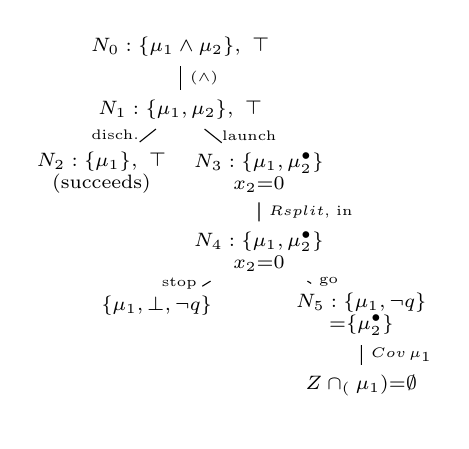
\begin{tikzpicture}[
  every node/.style={align=center, font=\scriptsize},
  level 1/.style={level distance=8mm},
  level 2/.style={sibling distance=20mm, level distance=8mm},
  level 3/.style={level distance=10mm},
  level 4/.style={sibling distance=26mm, level distance=8mm},
  level 5/.style={level distance=10mm},
  edge from parent/.style={draw,-}
]
\node {$N_0:\{\mu_1\wedge\mu_2\},\ \top$}
 child { node {$N_1:\{\mu_1,\mu_2\},\ \top$}
   child { node {$N_2:\{\mu_1\},\ \top$\\ (succeeds)}
     edge from parent node[left,font=\tiny,pos=.45]{disch.} }
   child { node {$N_3:\{\mu_1,\mu_2^\bullet\}$\\ $x_2{=}0$}
     child { node {$N_4:\{\mu_1,\mu_2^\bullet\}$\\ $x_2{=}0$}
       child { node {$\{\mu_1,\bot,\neg q\}$\\ $\CLOSED$}
         edge from parent node[left,font=\tiny,pos=.5]{stop} }
       child { node {$N_5:\{\mu_1,\neg q\}$\\ $\Ctx{=}\{\AX\mu_2^\bullet\}$}
         child { node {$Z\cap\Sat_\Ctx(\mu_1){=}\emptyset$\\ $\CLOSED$}
           edge from parent node[right,font=\tiny,pos=.5]{$\rlink{Cov}\,\mu_1$} }
         edge from parent node[right,font=\tiny,pos=.5]{go} }
       edge from parent node[right,font=\tiny]{$\rlink{Rsplit}$, in} }
     edge from parent node[right,font=\tiny,pos=.45]{launch} }
   edge from parent node[right,font=\tiny]{$(\wedge)$} };
\end{tikzpicture}}
\subcaption{$\mu_1\wedge\mu_2$: \UNSAT.}\label{fig:ex-unsat}
\end{subfigure}
\hfill
\begin{subfigure}[t]{0.49\textwidth}\centering
\resizebox{\linewidth}{!}{%
\begin{tikzpicture}[
  every node/.style={align=center, font=\scriptsize},
  level 1/.style={sibling distance=20mm, level distance=8mm},
  level 2/.style={level distance=10mm},
  level 3/.style={sibling distance=15mm, level distance=9mm},
  level 4/.style={sibling distance=20mm, level distance=9mm},
  level 5/.style={level distance=8mm},
  edge from parent/.style={draw,-}
]
\node {$N_0:\{\mu_1\},\ \top$}
 child { node (free) {$N_1:\{\,\},\ \top$\\ $\OPEN$}
   edge from parent node[left,font=\tiny,pos=.45]{disch.} }
 child { node {$N_2:\{\mu_1^\bullet\}$\\ $x_1{=}0$}
   child { node {$N_3:\{\mu_1^\bullet\}$\\ $x_1{=}0$}
     child { node {$\{\bot,\nu\}$\\ $\CLOSED$}
       edge from parent node[left,font=\tiny,pos=.5]{stop} }
     child { node {$N_4:\{\nu\}$\\ $\Ctx{=}\{\AX\mu_1^\bullet\}$}
       child { node {$N_5:\{\nu^\bullet\}$\\ $x_\nu{=}0$}
         child { node {$\{p,\EX\nu^\bullet\}$}
           child { node {$\{q\},\ x_\nu\in[1,2]$\\ $\OPEN$}
             edge from parent node[right,font=\tiny,pos=.5]{$\rlink{Delay}$, $\rlink{EX}$} }
           edge from parent node[right,font=\tiny,pos=.5]{$\rlink{Ugo}$} }
         edge from parent node[right,font=\tiny,pos=.5]{$\rlink{Cov}\,\nu$} }
       edge from parent node[right,font=\tiny,pos=.5]{go} }
     edge from parent node[right,font=\tiny]{$\rlink{Rsplit}$, in} }
   edge from parent node[right,font=\tiny,pos=.45]{launch} };
\draw[->,dashed] (free.west) to[out=200,in=160,looseness=3.4]
  node[left=3pt,font=\tiny]{stutter} ([yshift=-3pt]free.north west);
\end{tikzpicture}}
\subcaption{$\mu_1$ alone: \SAT.}\label{fig:ex-sat}
\end{subfigure}
\caption{Tableau runs, with $\nu=\tEU{p}{q}{[1,2]}$, $\mu_1=\mathrm{AG}_{[0,4]}\nu$,
$\mu_2=\mathrm{AG}_{[0,3]}\neg q$.}\label{fig:ex}
\end{figure}

\begin{example}[$\mu_1\wedge\mu_2$]\label{ex:unsat}
After $(\wedge)$, covering $\mu_2$ succeeds under the empty context and splits $N_1$
into a discharge child and a launch child $N_3$, which carries $\mu_1$ alongside the
pursuit. At $N_3$ the zone is the point $x_2{=}0$, so \ruleref{Rsplit} leaves only its
in-part; \ruleref{Runf_in} closes the stop child on $\bot$ and yields $N_5$, where the
context now forces $\neg q$ wherever $x_2\in[0,3]$.

Covering $\mu_1$ there fails. Computing $\Sat_\Ctx(\mu_1)$ unfolds it to a demand for
$\nu$ at the onset, and unfolding $\nu$ by \ruleref{Uunf} closes both branches:
\ruleref{Ustop} lands on $x_\nu\in[1,2]$, which coincides with $x_2\in[1,2]\subseteq[0,3]$,
so the node carries $q$ and $\neg q$; \ruleref{Ugo} defers with no deadline to cap it, and
once $x_\nu>2$ the window has passed with the stop never taken, so every repeat fails
acceptance condition~(i). Hence $\Sat_\Ctx(\nu)=\emptyset$ at this onset,
$Z\cap\Sat_\Ctx(\mu_1)=\emptyset$, and neither \ruleref{Cov} nor \ruleref{Covstar} applies:
$N_5$ closes and the formula is \UNSAT. The calculus never compares the two modalities
directly; it only brings $q$ and $\neg q$ into one goal set over overlapping zones.
\end{example}

\begin{example}[$\mu_1$ alone]\label{ex:sat}
Without $\mu_2$ nothing constrains $q$, so covering $\nu$ at $N_4$ succeeds and launches
its pursuit with $x_\nu$ reset. That pursuit shows how a window is entered: at $N_5$ the
zone is $x_\nu{=}0$, so \ruleref{Ustop} has empty zone and closes, and only \ruleref{Ugo}
survives, asserting $p$ and deferring $\EX\nu^\bullet$. The resulting node is saturated,
so \ruleref{Delay} advances the zone and \ruleref{EX} supplies the successor carrying
$\nu^\bullet$; at the first one with $x_\nu\in[1,2]$ the stop child is consistent and the
eventuality is fulfilled.

Meanwhile $\AX\mu_1^\bullet$ rides every successor, re-imposing $\mu_1$ across its window.
Once $x_1>4$ the after-part of \ruleref{Rsplit} drops $\mu_1^\bullet$, leaving a goal-free
node whose stutter loop is accepting: no until pursuit is active, so condition~(i) is
vacuous, and $x_1$ is extrapolated above $M{=}4$. The cycle can only live in this lapsed
tail, since inside the window the release's own split bounds $x_1$. The marking succeeds,
and reading it off gives a one-location automaton labelled $p$ with a $q$-successor
reachable within $[1,2]$ of each onset.
\end{example}
